\section{Sensores}
\label{sec:sensores}

El controlador no ve el estado; ve medidas. Un simulador que le entrega el
estado verdadero al controlador permite sintonías que el dron real no
tolera, porque oculta el ruido que amplifica el derivativo, el retardo que
come margen de fase y la vibración que satura los motores. El módulo
\cod{sensors.py} modela los sensores del proyecto PAE con valores de hoja de
datos, y cada medida se construye como
\begin{equation}
\text{medida} = \text{verdad} + \text{sesgo} + \text{ruido blanco} + \text{vibración},
\quad \text{entregada con retardo y a su propia tasa.}
\end{equation}
La IMU se muestrea a la tasa del lazo de control (\val{ctrlHz}~Hz,
$\Delta t=2$~ms).

\subsection{Ruido blanco y la densidad espectral}

Las hojas de datos dan el ruido como densidad espectral $N$ (unidad
por $\sqrt{\text{Hz}}$). Muestreado a $f_s$ con ancho de banda igual a
Nyquist, la desviación por muestra es
\begin{equation}
\sigma = N\sqrt{f_s/2} = N\sqrt{1/(2\Delta t)} .
\label{eq:ruido}
\end{equation}
Con los valores de la \cref{tab:sensores}, a 500~Hz el giroscopio tiene
$\sigma=\val{sgGyro}$~$^\circ$/s y el acelerómetro
$\sigma=\val{sgAccmg}$~m$g$ (\val{sgAcc}~m/s$^2$). Son cifras pequeñas: en un
dron real el ruido propio del MEMS lo tapa la vibración, y por eso esta es
configurable por separado.

\begin{table}[H]
\centering
\small
\caption{Parámetros de los sensores (\cod{SensorConfig}).}
\label{tab:sensores}
\begin{tabularx}{\textwidth}{>{\raggedright\arraybackslash}p{3.4cm}>{\raggedright\arraybackslash}X>{\raggedright\arraybackslash}p{4.6cm}}
\toprule
Sensor & Modelo & Fuente del valor \\
\midrule
Giroscopio (ISM330DHCX) & ruido $5$~m$^\circ$/s/$\sqrt{\text{Hz}}$; sesgo inicial $\mathcal N(0,0.3^\circ/\text{s})$ por eje; deriva de sesgo (paseo aleatorio) $0.005^\circ$/s/$\sqrt{\text{s}}$; retardo 2~ms & ruido: hoja de datos DS13012 \cite{ism330}; sesgo y deriva: supuestos típicos \\
Acelerómetro (ISM330DHCX) & ruido $60~\mu g/\sqrt{\text{Hz}}$; sesgo constante $\mathcal N(0,0.05~\text{m/s}^2)$; retardo 2~ms & ruido: DS13012; sesgo: supuesto \\
Vibración de hélices & $3^\circ$/s (giro) y 1.5~m/s$^2$ (acel.) a la velocidad de hover, 2 palas & supuesto (\cref{sec:vibracion}) \\
Magnetómetro (MMC5983MA) & $\vect m_B=\R\T\vect m_E+\vect b_{EMI}+\mathcal N(0,0.04~\mu\text{T})$, 100~Hz & ruido 0.4~mG RMS, hoja de datos \cite{mmc5983} \\
Barómetro (BMP180) & $h+$deriva$+\mathcal N(0,0.17~\text{m})$, 40~Hz, retardo 30~ms, deriva $0.002$~m/$\sqrt{\text{s}}$ & 0.02~hPa RMS en ultra alta resolución \cite{bmp180} $\approx0.17$~m; tasa, retardo y deriva: supuestos \\
Posición externa (mocap/RTK) & $\vect p+\mathcal N(0,0.01~\text{m})$, 100~Hz, retardo 10~ms & supuesto; Larotta \cite{larotta24} usa un sistema externo de este tipo \\
\bottomrule
\end{tabularx}
\end{table}

\paragraph{Sesgo del giroscopio.} El sesgo inicial se sortea una vez por
semilla y luego deriva como paseo aleatorio,
$b_{k+1}=b_k+\mathcal N(0,\sigma_{bw}\sqrt{\Delta t})$. Un sesgo de
$0.3^\circ$/s parece poco, pero integrado sin corrección son $18^\circ$ en un
minuto: es la razón de ser de los estimadores de la \cref{sec:estimadores}.

\subsection{Vibración a la frecuencia de paso de pala}
\label{sec:vibracion}

Cada hélice de dos palas ligeramente desbalanceada sacude el bastidor dos
veces por vuelta. El simulador lleva la fase $\varphi_i$ de cada rotor
(integrada con $\Omega_i$ en cada subpaso de física) y suma al giroscopio y
al acelerómetro
\begin{equation}
\delta\vect\omega_{vib} = A_g\sum_{i=1}^4\left(\frac{\Omega_i}{\Omega_h}\right)^2\sin(n_b\varphi_i)\,\vect d_i,
\qquad
\delta\vect a_{vib} = A_a\sum_{i=1}^4\left(\frac{\Omega_i}{\Omega_h}\right)^2\sin(n_b\varphi_i)\,\vect d'_i,
\label{eq:vib}
\end{equation}
con $n_b=2$ palas, $A_g=3^\circ$/s, $A_a=1.5$~m/s$^2$, $\vect d_i$ una
dirección unitaria aleatoria fija por rotor y $\vect d'_i$ la misma dirección
con las componentes permutadas cíclicamente. La amplitud escala con
$\Omega^2$ porque la fuerza centrífuga de un desbalance de masa crece con el
cuadrado de la velocidad. La frecuencia del tono es
\begin{equation}
f_{bp}=\frac{n_b\,\Omega}{2\pi}=\val{fbp}~\text{Hz en hover}.
\end{equation}

\paragraph{Por qué importa a 500~Hz.} Con la IMU muestreada a 500~Hz el
límite de Nyquist es 250~Hz. En hover el tono de 177~Hz cae por debajo y
se ve tal cual; la densidad espectral del giroscopio simulado
(\cref{fig:psd}) tiene su pico en \val{psdPeak}~Hz, y la frecuencia media que
reporta el simulador es \val{fvib}~Hz. El tono se mueve con el acelerador, y
para $\sigma>\val{sigNyq}$ ($\Omega>\val{wNyq}$~rad/s) pasa de Nyquist y se
\emph{repliega}: a acelerador máximo, los \val{fbpmax}~Hz reales aparecen a
$500-320.4=\val{alias}$~Hz (medido: \val{aliasMeas}~Hz). Un filtro notch fijo
deja de servir justo cuando el dron más exige a sus motores. Los
autopilotos comerciales muestrean el giroscopio a 1--8~kHz por esa razón; el
lazo de 500~Hz del firmware ESP32 del proyecto obliga a convivir con el
problema, y el simulador permite estudiarlo.

\begin{figure}[H]
\centering
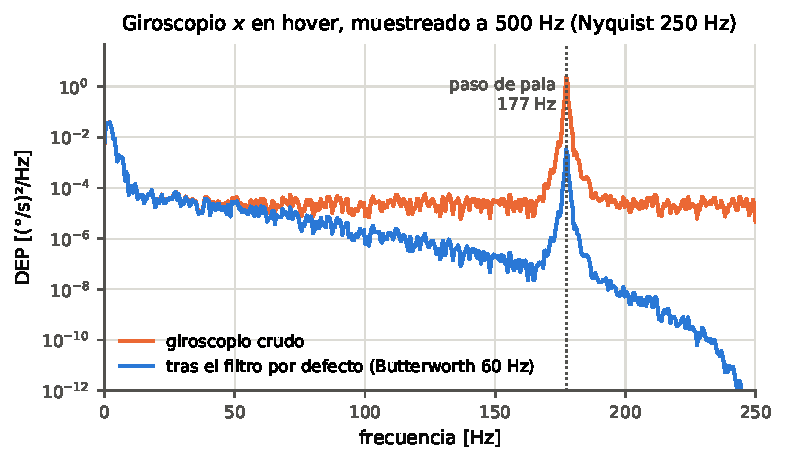
\includegraphics[width=0.78\textwidth]{psd_giroscopio_vibracion.pdf}
\caption{Densidad espectral del giroscopio $x$ en hover (simulador completo,
9~s, 500~Hz). El RMS del giroscopio crudo es \val{rmsRaw}~$^\circ$/s y, tras
el filtro por defecto (\val{filtroDef}), \val{rmsFilt}~$^\circ$/s.}
\label{fig:psd}
\end{figure}

\begin{supuesto}[Amplitud de la vibración]
Las amplitudes $A_g$ y $A_a$ y el espectro de un solo tono por rotor son
supuestos de orden de magnitud. El estudio de barridos (\cref{sec:barridos})
muestra que las conclusiones cualitativas sobre filtros no dependen de ellas,
pero los valores óptimos sí: antes de transferir una sintonía de filtro al
dron real hay que medir su espectro en hover y ajustar $A_g$.
\end{supuesto}

\subsection{Campo magnético}

El campo terrestre en NED geográfico se construye con intensidad $F$,
inclinación $I$ (positiva hacia abajo) y declinación $D$:
\begin{equation}
\vect m_E = F\,\big(\cos I\cos D,\ \cos I\sin D,\ \sin I\big)
= (\val{magN},\ \val{magE},\ \val{magD})~\mu\text{T},
\label{eq:magE}
\end{equation}
con $F=\val{magF}~\mu$T, $I=+\val{magI}^\circ$ y $D=\val{magDecl}^\circ$: el
World Magnetic Model 2025 evaluado para Valledupar (10.46$^\circ$N,
73.25$^\circ$O, unos 170~m de altura), la ciudad más cercana a la sede La
Paz, en la fecha 2026.75 (paquete \cod{pygeomag}). El campo cambia
lentamente con los años; para otra fecha o lugar se recalcula con el mismo
modelo o con la calculadora de NOAA. El EKF usa la misma inclinación para su
referencia magnética. La interferencia $\vect b_{EMI}$ la pone el módulo de
perturbaciones (\cref{sec:perturbaciones}) y afecta solo a la medida: el dron
no la siente, el estimador sí.

\subsection{Retardos y tasas}

Cada sensor tiene una línea de retardo (\cod{\_Delay}) de
$n=\max(1,\operatorname{round}(\tau/\Delta t))$ muestras de control: \val{dImu}
para la IMU, \val{dPos} para la posición externa y \val{dBaro} para el
barómetro. Magnetómetro, barómetro y posición se actualizan a su tasa y
mantienen el último valor entre actualizaciones; cada muestra lleva un
indicador \cod{*\_new} para que los estimadores solo corrijan con datos
nuevos.

\begin{nota}[Inicialización de las líneas de retardo]
Las líneas de retardo de la posición y del barómetro se construyen llenas
con el origen y altura cero, lo correcto para un despegue desde el suelo. Si
la simulación arranca en el aire (\cod{start\_airborne=True}),
\cod{Simulation.\_prime\_airborne} llama a \cod{SensorSuite.prime(x)}, que las
llena con el estado inicial; sin ese paso, durante los primeros 10~ms
(posición) y 30~ms (barómetro) los sensores reportarían ``dron en el origen,
en el suelo'' y el filtro de navegación saltaría la altura completa.
\end{nota}
